%-*- coding:UTF-8 -*-
%gougu.tex
%高温半导体材料调研
%编译环境xelatex->bibtex->xelatex->xelatex
\documentclass[UTF8, twocolumn]{ctexart}
\usepackage{graphicx}           %图表环境
%\usepackage{amsmath}            %公式环境
\usepackage{geometry}
\geometry{a4paper,left=2cm,right=2cm,top=2cm,bottom=2cm}
\usepackage[format=hang,font=small,textfont=it]{caption}
\CTEXsetup[format={\Large\bfseries}]{section}  %标题居左
\usepackage{abstract}
\renewcommand{\abstractname}{}
\usepackage{stfloats}
\usepackage{cite}
\usepackage{fancyhdr}
\renewcommand{\headrulewidth}{0.4pt}


\title{\fangsong 高温半导体材料调研}
\author{\kaishu 王展鹏}
\date{\today}

\bibliographystyle{unsrt}           %样式同plain,只是按照引用的先后排序

\begin{document}

\twocolumn[
\maketitle
\thispagestyle{fancy}

\begin{onecolabstract}
    \zihao{-4}\kaishu\noindent{摘要} 这是高温半导体材料的调研内容,先写上东西再说,摘要很长很长很长很长很长

\end{onecolabstract}
]

\section{引言}

    超导体(Superconductor),指可以在特定温度以下,呈现电阻为零的导体。零电阻和完全抗磁性是超导体的两个重要特性。超导体电阻转变为零的温度,称为超导临界温度,据此超导材料可以分为低温超导体和高温超导体。虽然是高温超导,其实是相对于绝对零度而言,因此其温度可以远低于冰点摄氏$ 0 ^\circ C$。当温度很低时,超导体并没有太大的应用,科学家一直在寻求提高超导材料的临界温度,称之为“高温超导体”。

    \begin{figure*}[hb]
        \centering
        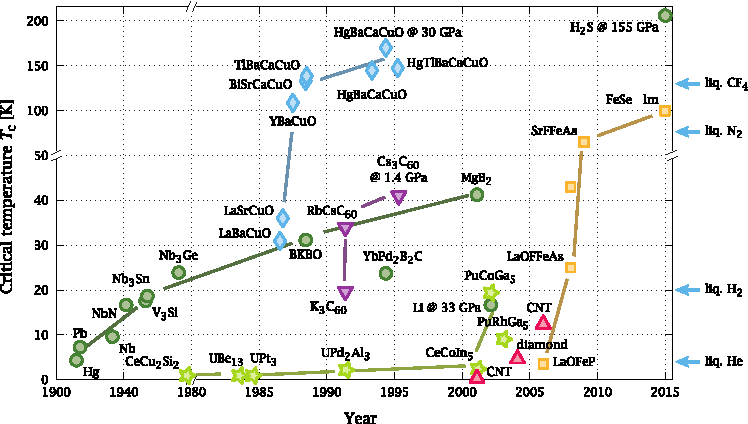
\includegraphics[scale=1.2]{image/Timeline_of_Superconductivity_from_1900_to_2015.pdf}
        \caption{自1911年首次发现以来,各种超导材料的超导临界温度概述}
        \label{fig:image1}
    \end{figure*}

    \subsection{超导体演化历史}
    1911年,荷兰科学家海克·卡末林·昂内斯用液氦冷却汞,发现当温度下降到绝对温标$4.2K$时水银的电阻完全消失,这种现象称为超导电性,将此温度称为临界温度。

    1933年,瓦尔特·迈斯纳和罗伯特·奥克森菲尔德两位科学家发现,如果把超导体放在磁场中冷却,则在材料电阻消失的同时,磁感应线将从超导体中排出,不能通过超导体,这种现象称为抗磁性。经过科学家的努力,磁电障碍已被跨越,下一个难关是突破温度障碍,寻求高温超导材料。

    2015年,德国普朗克研究所的V.Ksenofontov和S.I.Shylin研究组创下了新的超导温度记录:$203K$。其物质为硫化氢。

    图\ref{fig:image1}即为已发现的各种超导材料的超导临界温度概述\cite{Ray2016}。

    \subsection{高温超导体简介}

    高温超导体(High-temperature superconductors)是超导物质中的一种族类,具有一般的结构特征以及相对上适度间隔的铜氧化物平面。它们也被称作铜氧化物超导体。此族类中一些化合物中,超导性出现的临界温度是已知超导体中最高的。不同铜氧化物在常态(以及超导态)性质之间具有共同的特征;这些性质中,许多无法以金属的传统理论来解释。

\section{高温超导发展简史}

    铜氧化物超导体在实验上是由卡尔·米勒及约翰内斯·贝德诺尔茨首度发现。

    1987年,来自台湾的美国物理学家吴茂昆和朱经武在钇钡铜氧系材料上把临界温度提高到了$90K$以上。以吴茂昆为第一作者的论文\cite{PhysRevLett.58.908}发表以来已获期刊引用论文五千多次,史上第一次超越液态氮沸点“温度壁垒”将超导温度从$30K$提升到$90K$,被称为超导体领域30年来最重要的先驱之一。

    2015年,物理学者发现,硫化氢在极度高压的环境下(至少150$GPa$,也就是约150万标准大气压),约于温度203$K$时会发生超导相变\cite{drozdov2015conventional}。

    2018年,德国化学家发现十氢化镧有超导性出现,是目前已知最高温度的超导体。

    十氢化镧是镧和氢形成的氢化物之一,化学式为$LaH_{10}$,是一种多氢化物或超氢化物,有望用作高温超导体。它的超导转变温度$T_c$为约250 $K$$(150 GPa)$,是2019年记录新高。其合成需要约160 $GPa$以上的压力。在1,000$ K$能够制得立方晶系的晶体,在室温得到的是六方晶系的晶体\cite{drozdov2019superconductivity}。

\section{国内外高温超导材料发展现状}

\section{技术及其特点}

\section{我们的工作}

\section{总结}

\kaishu
\addcontentsline{toc}{section}{参考文献}
\bibliography{main.bib}


\end{document}